\section{Wichtige Begriffe}
\subsection{Repository}
Unter einem Repository versteht man ein zentrales, auf einem Server lagerndes Archiv, das über die gesamte Versionsgeschichte jeder Datei, die im Repository abgelegt wurde, verfügt.\\
Da man in der Regel für jedes Projekt ein eigenes Repository benutzt, ist ein Subversion-Server in der Lage mehrere Repositories zu verwalten.\\
Zum Bearbeiten der versionierten Dateien lädt man sich eine lokale Arbeitskopie aus dem Repository und lädt anschließend die veränderten Dateien in das Repository.
\subsection{Revision}
Im jedem Repository gibt es die sogenannte Revisionsnummer. Beim Anlegen eines Repositories beträgt sie null und wird bei jeder eingereichten Änderung um 1 inkrementiert. Für jede versionierte Datei wird zusätzlich die Revisionsnummer der letzten Bearbeitung gespeichert.\\
Durch Angabe einer Nummer lässt sich die Version einer Datei eindeutig bestimmen und so auch der Zustand einer Datei oder des gesamten Projektes zu einem bestimmten Zeitpunkt wiederherstellen.\\
Die aktuellste des Repository nennt man auch \emph{head} und die lokale, noch nicht eingereichte Revision, heißt \emph{base}.
\subsection{Verzeichnisstruktur}
Unabhängig von der Art des Projektes hat sich eine Verzeichnisstruktur etabliert, die mehrere Entwicklungsstränge ermöglicht.\\
Der Hauptentwicklungszweig lagert in \emph{trunk}, Nebenzweige werden in \emph{branch} abgelegt und \emph{tag} enthält benannte Versionen.\\
Da in Subversion beim kopieren einer Datei, nicht die Datei kopiert wird, sondern nur ein neuer Verweis in der Datenbank angelegt wird, ist es möglich ohne zusätzlichen Speicherbedarf Dateien zu kopieren und deren Versionsgeschichte zu erhalten. Möchte man nun eine eine benannte Version (bspw. ein Release Candidate o.ä.) erstellen, reicht es mit Hilfe von Subversion das Projekt aus \emph{trunk} nach \emph{tag} zu kopieren und dort umzubennen. Subversion legt dabei nur eine Verknüpfung unter dem neuen Namen mit der Versionsgeschichte der Originaldateien an.\\
Gleiches geschieht beim Erstellen eines neuen Entwicklungszweiges in \emph{branch}.
\section{Konflikte}
\begin{figure}[!htb]
\centering
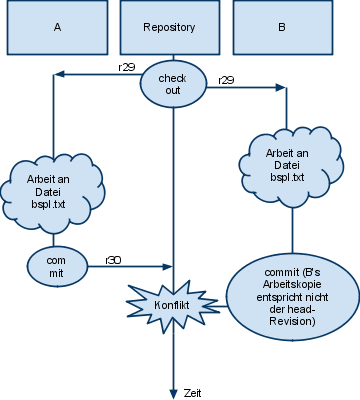
\includegraphics[width=0.7\textwidth]{konflikt}
\caption{Konflikt beim gleichzeitigen Bearbeiten einer Datei (Quelle: eigene Darstellung).}
\label{fig:konflikt}
\end{figure}
Subversion erlaubt das gleichzeitige Arbeiten mehrerer Personen an der selben Datei. Dies führt zwangsläufig zu Konflikten wie Abbildung \ref{fig:konflikt} zeigt. Subversion bietet hierfür zwei Lösungen an.
\subsection{Merge}
In Abbildung \ref{fig:konflikt} kann B nicht einfach seine Änderungen commiten, da dies alle Änderungen, die A gemacht hat, verwerfen würde. Daher ist B gezwungen die im Konflikt stehenden Dateiversionen zu verschmelzen (zu mergen). Dies kann automatisch (bsplw. wenn sich die Veränderungen nich gegenseitig beeinflussen) oder von Hand geschehen. Um dies zu Vereinfachen gibt es eine Vielzahl Tools die einen synoptischen Vergleich der Dateien ermöglichen und die Unterschiede visualisieren.

\subsection{Locks}
Locks eigenen sich besonders für binäre Dateien, bei denen ein synoptischer Vergleich der beiden in Konflikt stehenden Dateien nicht möglich ist.\\
Um Konflikte zu Verhindern wird bevor die Datei bearbeitet wird eine Sperre (der sogenannte Lock) für die Datei angefordert. Alle anderen Personen können ab diesem Zeitpunkt zwar die Datei lesen und bearbeiten, allerdings nicht commiten. Erst mit dem nächsten Commit des Lock-Inhabers wird die Datei wieder für andere freigegeben.\\
Da man eine von jemand Anders gesperrte Datei in seiner Arbeitskopie beliebig verändern kann und über ein Lock nur bei einem versuchten Commit informiert wird, empfiehlt es sich vor jedem Bearbeiten den Status einer Binärdatei zu überprüfen um unnötige Arbeit zu verhindern.

\section{Die Kommandozeile}
